%\section*{Simplified formalism}
A much shorter version has already been derived\scite{Litzen1991} with the assumptions $L_{23} = L_2 
+ L_3$. %and $b(L) \approx b(L_{12}) = b_L$.
In addition, in this model the extrapolated channel breadths $b_0$ and $\bL$ are used. They are given with
\begin{equation}
b_0 = 2e_2(0) = b_1+\frac{L_1}{L_2}\bDelta 
\end{equation}
and
\begin{equation}
b_L = 2e_2(L) 
= b_1+\frac{L_1}{L_2}\bDelta - \frac{L}{L_2}\bDelta 
= b_1-\frac{L_{23}}{L_2}\bDelta 
\end{equation}
Here, 
\begin{equation}
\begin{array}{lll}
\tvoid &= & \frac{\Vappgeo}{\Vc} \ln{
  \left(
  1 + \frac{\Vc}{\Ve}
  \left(
  1 - \frac{
    w 
    \left(
    b_0 z_0 
    - \frac{
      z_0^2 \bDelta
    }{
      2L} 
    - Y
    \right)
  }{\Vappgeo}
  \right)
  \right)}
\\\addlinespace
&= &\frac{\Vappgeo}{\Vc} \ln{
  \left(
  1 + \frac{\Vc}{\Ve}
  \left(
  1 - \frac{
    b_0 z_0 
    - \frac{
      z_0^2 \bDelta
    }{
      2L
    } 
    -  Y
  }{
 \int_{0}^{L} b(z) \diff z 
}
  \right)
  \right)}
\end{array}
\end{equation}
\begin{figure}[H]
  \begin{center}
    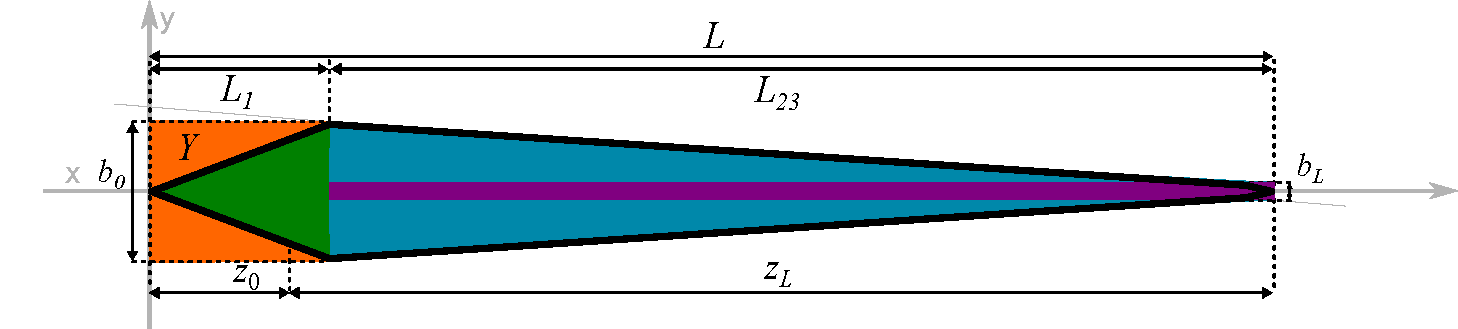
\includegraphics[width=\linewidth]{./images/fffSimplified.pdf}
    \vspace*{-3ex}    
  \end{center}
  \caption[Total area of an AF4 channel in the simplified model]{
    Total area of an AF4 channel in the simplified model.}
  \label{fig:fffSimplied}
\end{figure}
With these assumptions, the channel surface $\AL$ is computed as
\begin{equation}
\AL = \int_{0}^{L} b(z) \diff z 
= 
\intGreenBox{\ensuremath{\frac{1}{2} b_1 L_1}}
+ 
\intPurpleBox{\ensuremath{b_2 L_{23}}}
+
\intBlueBox{\ensuremath{\frac{1}{2} (b_1-b_2) L_{23}}}
\end{equation}
$Y$ is the enclosed area of the elongation from,
$e_2(x)$ y-axis and $e_1(x)$ and its symmetrical counterpart 
%(Fig. \ref{fig:fffApprox1} and \ref{fig:fffApprox2}). 
(Fig. \ref{fig:fffSimplied})
It can be calculated by simple geometrical considerations as 
\begin{equation}
\intOrangeBox{\ensuremath{ Y \hspace{-4ex}\phantom{\left(\frac{1}{2}\right)} }} 
= \intOrangeBox{\ensuremath{ 2\cdot\left(\frac{1}{2} L_1 b_1 \right)
  + 2\cdot\left( \frac{1}{2} L_1 \left( b_0 - b_1 \right) \right) }} 
=\intOrangeBox{\ensuremath{ L_1 b_0 \hspace{-4ex}\phantom{\left(\frac{1}{2}\right)} } }
%= \intOrangeBox{\ensuremath{ }} 
%\intOrangeBox{\ensuremath{\displaystyle\phantom{\hspace{-4ex} \int_0^{L1}} Y  }} 
%= \intOrangeBox{\ensuremath{\displaystyle 2 \int_0^{L1}e_2(2)\diff x - \frac{1}{2}b_1L_1  }}Z
%= \intOrangeBox{\ensuremath{ 2 \cdot \frac{1}{2} e_2(0) L_1 }} = 
%\intOrangeBox{\ensuremath{ \frac{1}{2}\left( b_0 + \frac{L_1}{L_{23}} \bDelta \right) L_1 }}
\end{equation}

The channel volume in the simplified model is also given by elementary geometry:
\begin{equation}
  \Vappgeo = \wappgeo \AL
\end{equation}

\begin{comment}
The area, which is relevant for separation, could also be calculated according to the geometrical considerations from 
above.
In this simplified version, the proximal and distal focusing cases have to be distinguished:
\subsubsection*{Distal focusing with \bm{$z_0  \geqq L_1$}}
In this case, only the relevant part on the elongated surface is considered (Fig. \ref{fig:fffApprox1}).
%\FloatBarrier
\begin{figure}[h]
  \begin{center}
    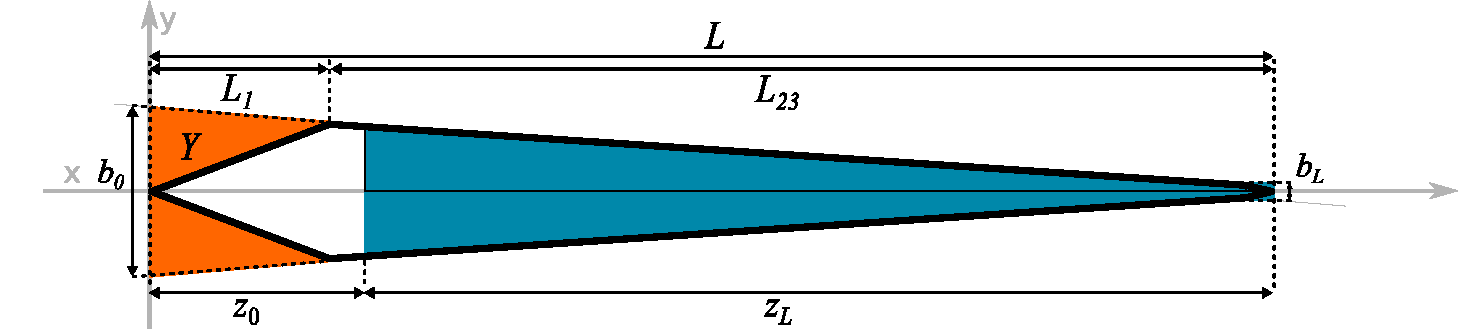
\includegraphics[width=\linewidth]{./images/fffApprox1.pdf}
    \vspace*{-3ex}    
  \end{center}
  \caption[Passed area section - distal focussing, simplified approximation]{
   Simplified model of relevant passed area sections acccording to literature\scite{Litzen1991}  in case of a distal 
   focusing 
   point. }
  \label{fig:fffApprox1} 
\end{figure}
\begin{equation}
\frac{\Vappgeo}{w} = 
 \int_{z_0}^{\zL} b(z) \diff z = 
\frac{1}{2}
%\left( b_0 - b_L  \right)
\bDelta
\left( L_{23} - z_0 \right) 
\end{equation}
\FloatBarrier
\subsubsection*{Proximal focusing with \bm{$z_0 < L_1$}}
In this case, the additional space on the left part has to be considered as well (Fig. \ref{fig:fffApprox2}).
\begin{figure}[H]
  \begin{center}
    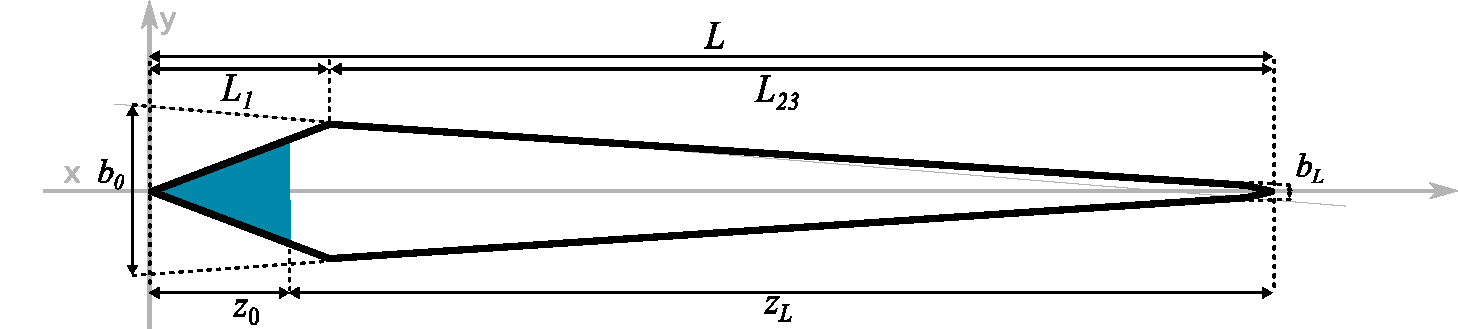
\includegraphics[width=\linewidth]{./images/fffApprox2.pdf}
    \vspace*{-3ex}    
  \end{center}
  \caption[Passed area section - distal focussing, simplified approximation]{
    Simplified model of relevant passed area sections acccording to literature\scite{Litzen1991} 
   in case of a proximal focusing 
    point.}
  \label{fig:fffApprox2}
\end{figure}

\begin{equation}
\frac{\Vappgeo}{w} = 
 \int_{z_0}^{\zL} b(z) \diff z = 
\intGreenBox{ \ensuremath {\frac{b_0}{2 L_1}  (L_1^2-z_0^2) }}
+ \intBlueBox{ \ensuremath { \frac{1}{2} 
    %\left( b_0 - b_L  \right)
    \bDelta
      L_{23} } }
\end{equation}

\end{comment}
